\chapter{Networking Software Development Environment}
\label{chapter4}
    % Broadband in rural situations is limited due to reasons explained in Chapter 3
    % In addition to creating and testing new topologies, other methods can be used to maximize the deliverable bandwidth
    % In this case, giving users bandwidth in an intelligent manner can allow the network to perform better
    % Utilizes the OVERCOME testbed from Chapter 3
The second scenario EMANE was used for was the development of an intelligent resource allocation program.
The goal of the network topologies presented in Chapter~\ref{chapter3} were to deliver greater amounts of connectivity to underserved rural communities.
Introducing new networking hardware is one way of achieving this goal, but another potential for increasing the usability of the Internet is to better allocate resources in an intelligent manner.
By using the EMANE testbed developed in the previous chapter, an accurate environment for developing this software can be created.
Testing inside an emulated EMANE environment allows the software to still act on an accurate network without needing to be deployed to users.
Developing in a production environment could have potentially several issues, such as violating the privacy concerns of users, or diminishing the quality of service a user experiences.
This chapter will present the initial creation of a tool to achieve the goal of more intelligently distributing network resources.

\section{Intelligent Method of Bandwidth Distribution}
The original proposal for the software developed in this chapter was to utilize machine learning tools to create a model that would be able to allocate resources in a network with high efficiency.
This was deemed to be too complex of a first step and so instead a heuristic approach was decided upon with a special focus on determining if EMANE could make an adequate development environment for this tool.
The primary motivation behind the intelligent router program was the idea that using an identical, static bandwidth cap for each house on the network is not efficient, and even a scheme were certain houses are able to have higher reservations (similar to what most ISPs presently use) would leave too much bandwidth unused.
Ideally the only time the network should not be at 100\% usage is when there are enough users online to bring it to full capacity.
There should not be a situation where a user cannot access resources simply because they are allocated to another user, and that user is not using them.\par
To facilitate the development of this tool, the OVERCOME EMANE testbed from Chapter~\ref{chapter3} was modified to create a better environment to develop in. 
Figure~\ref{pfsense_dev} shows the modified environment.
The primary difference is the removal of the mmWave model and instead directly connecting the router to the Internet (or other upstream data source).
The intelligent router was only concerned with the distribution of network resources from the aggregated central point, and as such the characteristics of the mmWave backhaul were deemed unnecessary to model.
The program was eventually deployed to the full OVERCOME EMANE testbed before deployment to hardware, but this was a very minor test to ensure the behavior did not change between virtual environments.
\begin{figure}[!ht]
    \centering
    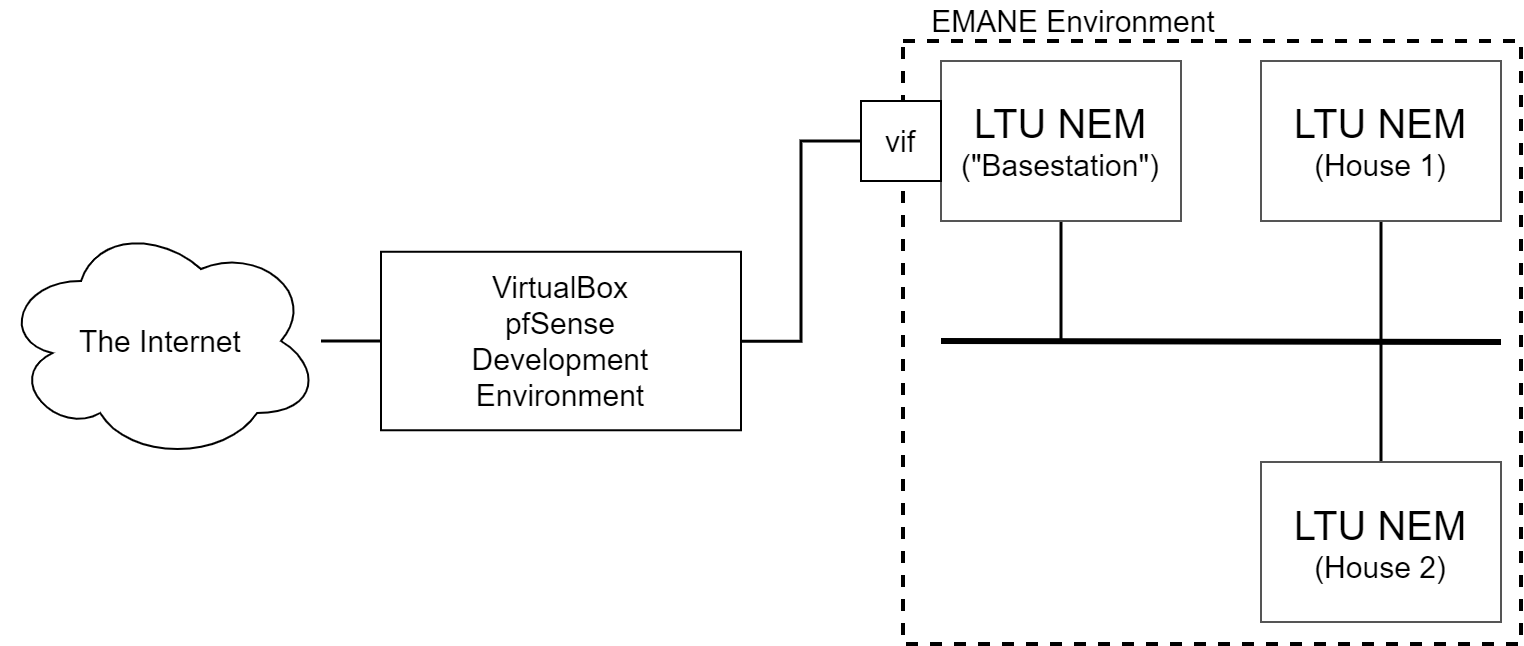
\includegraphics[width=\textwidth,keepaspectratio]{Images/Chpt4/pfsense_dev.png}
    \caption{The modified OVERCOME EMANE testbed used for development of the intelligent router program. The primary modification is the removal of the mmWave environment.}
    \label{pfsense_dev}
\end{figure}

\section{Implementing the Software}
The algorithm for allocating bandwidth consists of two major stages: (1) classification of the current state of the network, and (2) allocation to modify the state of the network.

\subsection{Stage 1: Classification}
    % Want to classify each host's current upload/download usage
        % Used tool: iftop to get average usage over 2 seconds, record usage every 6 seconds (10 times per minute)
In order to determine how bandwidth should be distributed to users, the program first needed to be aware of the current state of the network.
There were a few different tools that were considered to determine the current usage of each host on the network.
Because of software was to run on pfSense, this greatly limited the available software.
A majority of the usable packages were only the ones made available through the pfSense add-on library.
Since the add-on programs and router could not tolerate any possible security vulnerabilities, tools had to be extensively validated before being added to the plugin library.
On top of this most of the software made available by pfSense was graphical (as pfSense is effectively a graphical layer for FreeBSD~\cite{freebsd}).
Needing a tool that would output to the console, or have a redirectable output that could be intercepted by Python \textit{iftop}~\cite{iftop} was selected.
This tool takes the average bandwidth traveling through an interface and outputs the values to the terminal.
Figure~\ref{iftop_out} shows an example output of this tool.
This data was used to aggregate the IP addresses and upload and download bandwidths (in Kbps) for each house present on the network.
Figure~\ref{log_file} is an example of a log file that shows the data generated by \textit{iftop}. (IP addresses have been censored for user privacy).\par
\begin{figure}[!ht]
    \centering
    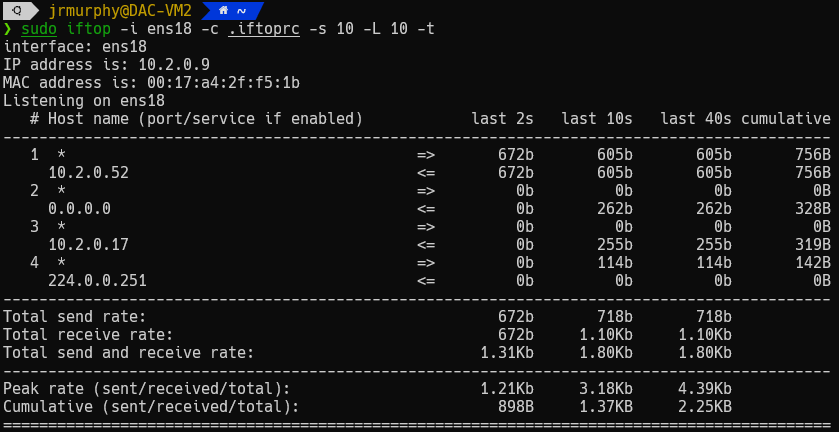
\includegraphics[width=\textwidth,keepaspectratio]{Images/Chpt4/iftop_util.png}
    \caption{An example of the output of the \textit{iftop} utility used to measure bandwidth on the OVERCOME network.}
    \label{iftop_out}
\end{figure}
\begin{figure}[!ht]
    \centering
    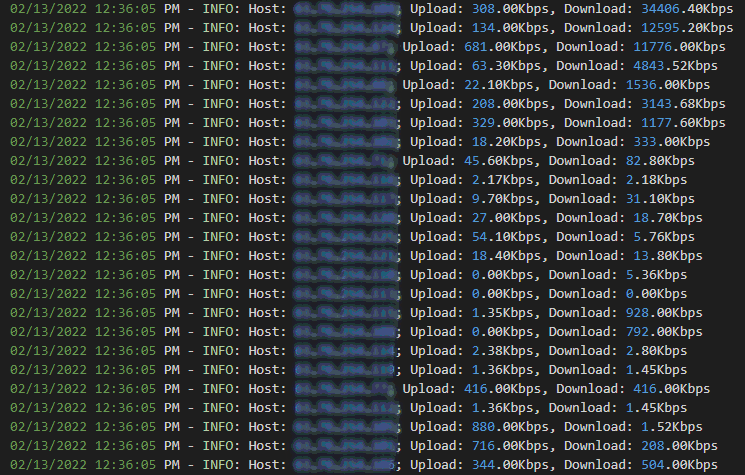
\includegraphics[width=0.8\textwidth,keepaspectratio]{Images/Chpt4/LogFile.png}
    \caption{An example of the data output but the classification stage of the intelligent router program. IP addresses have been censored for privacy.}
    \label{log_file}
\end{figure}
    % Use this classification to create priority tiers that influence how users get more bandwidth/bandwidth taken away
    % What is the rationale behind these priorities (study on what types of behaviors use what types of bandwidth)
The bandwidth data was then used to classify each host into a priority level.
In order to not invade the privacy of the users on the network, it was decided that priority levels should not be determined based on the user's specific activity and traffic type.
To identify what services each user was using would require examining the user's traffic which is not only computationally inefficient, but also a breach of privacy.
In addition to this, our algorithm is not in a position to determine what type of traffic is more important.
Identifying the difference between a Zoom meeting and a Netflix stream does not indicate which one should be prioritized and this was not a decision we were in a position to make.
Instead, the four created priorities were based on the amount of bandwidth being used.
This would give some insight into what the user was doing, and since high bandwidth activities are typically more sensitive to limited datarates, it made sense to prioritize those users.
Table~\ref{priority_table} shows the priority classifications, as well as the thresholds for ``high'' and ``low'' bandwidths.
The potential was also discussed for adding specific priorities to better control large uploads or downloads, but was never implemented.\par
\begin{table}[!ht]
\centering
\caption{Priority groups for the intelligent router, based on user bandwidth behaviors}
\begin{adjustbox}{width=0.6\textwidth, center=\textwidth}
    \begin{tabular}{r|cc}
    \multicolumn{1}{c|}{} & Download Behavior & \multicolumn{1}{l}{Upload Behavior} \\ 
    \hline
    Priority 1 & High ($>$5Mbps) & High ($>$200Kbps) \\
    Priority 2 & High ($>$5Mbps) & Low ($>$200Kbps)\\
    Priority 3 & Low ($<$5Mbps) & High ($>$200Kbps)\\
    Priority 4 & Low ($<$5Mbps) & Low ($>$200Kbps)
    \end{tabular}
\end{adjustbox}
\label{priority_table}
\end{table}
Once the priorities were assigned, the final step was to flag all hosts that needed reallocation.
The criterion for receiving reallocation was having a current average usage that was within 5\% of the currently set cap.
Meeting this criterion would indicate to the allocation stage that the house should receive more bandwidth (if possible).
The logic for this reallocation is discussed in the next subsection.
Figure~\ref{classification} provides an overview of the classification process.
The full source code for the classification stage of the router can be found in Appendix~\ref{appendixb}.
\begin{figure}[!ht]
    \centering
    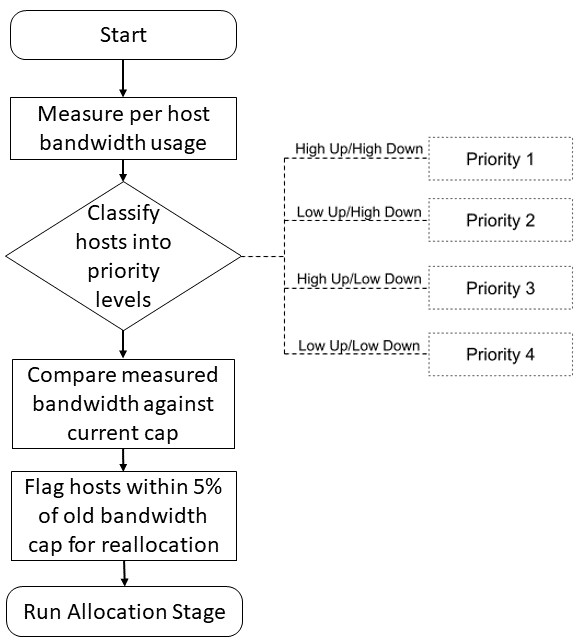
\includegraphics[width=0.5\textwidth,keepaspectratio]{Images/Chpt4/Flowchart_Classification_Updated.png}
    \caption{An overview of the algorithm that operates to classify each host on the network as a part of the intelligent router program.}
    \label{classification}
\end{figure}

\subsection{Stage 2: Allocation}
    % Create these modifications to move bandwidth caps up and down via pfSense limiters
Once the classification stage was complete, the allocation stage would run.
This stage read the data created by the previous stage and acted on it to impact the network and change the amount of bandwidth an individual house was able to use.
The primary decisions made while designing the allocation stage related to the safety measures put in place to ensure no user was allowed too much or too little bandwidth.
Since the algorithm was set up to continually take and give bandwidth, checks needed to be put in place to ensure a single house was not able to accumulate all the bandwidth, starving the rest of the hosts.
After evaluating the average usages for the network, the minimum value a house could have was set to 7.5Mbps.
This value was a rather conservative estimate and in all likelihood could have been set lower, but it did not impact the efficiency of the algorithm.\par
Once measures were put in place to protect the network, the method with which homes were limited had to be decided upon.
Since the algorithm implementation was running alongside pfSense, we had to be careful that the method we used to set limits would not be overridden by the primary router software.
To ensure this, we used pfSense's Limiters, a group of settings that could be assigned to a firewall rule to ensure a maximum throughput for any traffic caught by the rule.
This method worked well because each house could be assigned a firewall rule based on its IP address.
Any traffic destined to that IP address would pass through the limiter.
Additionally, because these settings were stored in the main configuration XML file, the Python script running the algorithm could easily edit and update the file, instead of trying to fight against the default configuration.\par
With these design decisions out of the way, several steps were put in place to allocate traffic.
The first step was to look at the total amount of bandwidth allocated and determine if the network was at saturation.
This was done by keeping a record of the sum of all allocations that was then compared against the known network total.
If bandwidth was available, the algorithm would proceed to increase every flagged host's bandwidth cap by 5Mbps.
If there was no extra bandwidth available, lower priority hosts that did not require as high limits would have their caps lowered, and the additional bandwidth could be redistributed.
Once all flagged hosts either had their caps raised, or were deemed unable receive more bandwidth, the program would wait six seconds before returning to the classification stage.
This waiting period is primarily to account for inefficiencies in the pfSense system.
Since pfSense was directly being used to change bandwidth caps, a small waiting period was required to allow the values to propagate through the system.
The full behavior of the allocation stage can be seen below in Figure~\ref{allocation}, and the full source code for the allocation stage of the router can be found in Appendix~\ref{appendixb}.
\begin{figure}[!ht]
    \centering
    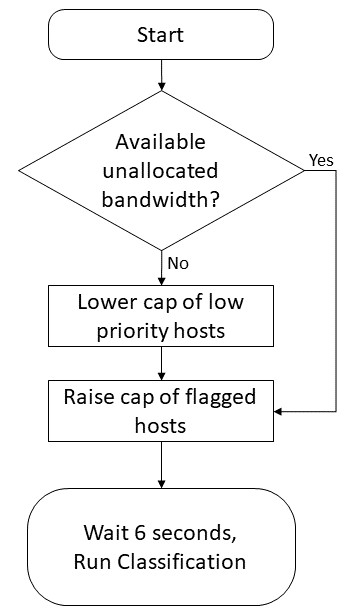
\includegraphics[width=0.4\textwidth,keepaspectratio]{Images/Chpt4/Flowchart_Allocation_Updated.png}
    \caption{An overview of the algorithm that operates to allocate bandwidth to each host on the network as a part of the intelligent router program.}
    \label{allocation}
\end{figure}

\section{Effectiveness of the Program}
    % Is EMANE effective?
Whether or not EMANE makes an appropriate environment to develop a tool similar to this is difficult to answer from the observed data and results.
One of the primary benefits of developing in EMANE is that it is a closed environment that protects the program and developer from errors effecting the quality of a network.
If the tool were to be developed in production, any small configuration error could easily result in taking down a network many people rely on.
Conversely, developing on a generic computer, or a router connected to only a very limited number of hardware devices does not provide the traffic or tools necessary to test the behavior.
By operating in EMANE, any number of ``houses'' can be connected downstream from the router, the amount of traffic being created at once and which hosts the traffic comes from is controllable, and the attributes of the communication medium can be modified.\par
This makes development very convenient, but should not be used as catch-all solution.
One of the major problems discovered during development is that the generated test traffic did not resemble the behavior of the real user traffic enough.
Traffic generated by a test tool such as \textit{MGEN} is typically not dynamic enough to mirror the behavior of an individual, let alone an entire household.
Extend this to covering the entire network, and generating test traffic that is accurate for five or ten households is a difficult task.\par
One solution attempted during the development of the tool, was to use a packet capture (in the form of a PCAP file) to record the traffic of consenting users and play it across the network.
The problem that was found with this solution was that different demographics will have drastically different traffic usage behavior.
The Internet usage of a New England college student does not necessarily match that of an adult in a rural area such as Missouri.
This became a problem during testing as the algorithm was reacting slower to bandwidth needs than in testing, as the high usages were more sporadic so the averaging approach at classification tended to trend lower than required.\par
    % Only deployed for an initial iteration due to network issues
        % No revisions made, only tested the most basic behavior
    % Not enough traffic/users on the network for meaningful data
        % At no point during any test was total network utilization above 50%, can't take bandwidth from users to give to others if there is always a pool
    % Ways to modify/fix the experiment and test environment to create a meaningful test
The other major result from the testing of the router, was the discovery that effective testing of a program similar to this requires an ideal environment to test in.
The OVERCOME hardware network was not constrained enough due to the small number of houses connected.
An attempt was made to constrain the network during testing, but was overall unsuccessful.
The hardware testing schedule proceeded as follows:
\begin{itemize}
    \item \textbf{Week 1:} No artificial bandwidth limits, no intelligent program.
    \item \textbf{Week 2:} All homes restricted to 25Mbps download in an attempt to create a lower max network capacity.
    \item \textbf{Week 3:} Homes were assigned dynamic restrictions based on the algorithm.
\end{itemize}
\begin{figure}[!ht]
    \centering
    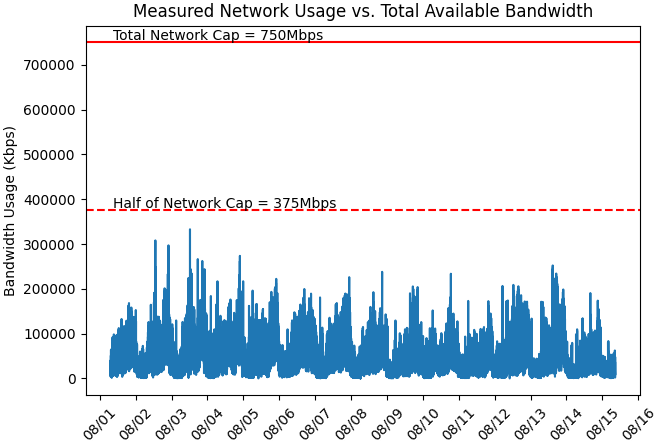
\includegraphics[width=0.8\textwidth,keepaspectratio]{Images/Chpt4/Network_Usage.png}
    \caption{The total network usage for thirty houses in the Project OVERCOME testbed during weeks 2 and 3 of the intelligent router test.}
    \label{max_usage}
\end{figure}
Figure~\ref{max_usage} shows the total usage of the network during each classification iteration for the entire week 2 and 3 testing period.
As can be seen by the blue traffic data, at no point during the two-week period was the usage in the network even at 50\% capacity.
This caused the intelligent algorithm to never have to remove bandwidth from a user to give to another user, eliminating the point of the program.
The artificial cap on the network also could not be lowered further, because the individual households would have such a low base restriction that users would be barely able to use the Internet during the control period.
With the project near completion, it was determined that another test could not be run, and the algorithm would have to remain unfinished as future work.\par
However, one positive result from the test was data confirming that a stratification of usage existed on the network.
By confirming that there is a distribution of users that use a significant amount of bandwidth and users that use little, it supports the core concept of the algorithm that a flat distribution cap on a network, while fair, is not the most efficient use of resources.
Figure~\ref{usage_compare} shows an example of two houses on the network. The top house with much higher usage, and the bottom house with less usage.
\begin{figure}[!ht]
    \centering
    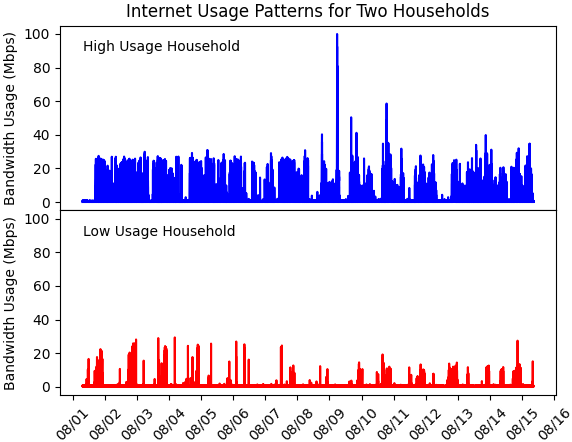
\includegraphics[width=0.8\textwidth,keepaspectratio]{Images/Chpt4/Network_Compare.png}
    \caption{The total network usage for thirty houses in the Project OVERCOME testbed during weeks 2 and 3 of the intelligent router test.}
    \label{usage_compare}
\end{figure}

\section{Chapter Summary}
This chapter outlined the process for designing a piece of networking software while using EMANE as the network environment for development.
More specifically, a program that sought to heuristically allocate network resources in an intelligent manner was outlined.
The specifics of the environment the tool was developed in were highlighted and the behavior of the algorithm explained.
The chapter finalizes by outlining lessons learned from the development and testing of the tool, with the main takeaway being emulation environments need to also validate the behavior of the test traffic, in addition to the models provided and used.